\chapter{Experimental Results} \label{chap:experimental-results}
Now it will be presented the experimental results obtained using the methodology explained in the previous chapter.
First it will be described the Hardware and Software setup used during the experiments. Next, it will be explained how the presented methodology can be applied considering a typical robotic system developed for mobile robot navigation in a warehouse scenario.

\section{Setup}
The main technicals specifications of the \textit{Host} and the embedded device used during the experiments are shown in table \ref{tab:tech-specs-host} and in table \ref{tab:tech-specs-tx2} respectively. 

\begin{table}[htbp]
	\centering
	\begin{tabularx}{\linewidth}{|l|X|}
		\hline
		\rowcolor{Gray}
		Hardware         & Model                                   										   \\
		\hline
		Processor        & Intel(R) Core(TM) i5-7400 CPU @ 3.00GHz  \\
		Storage          & SATA 500GiB                             									 \\
		Memory           & 16GiB                                   											\\
		GPU              & NVIDIA GeForce GTX 980                  						   \\
		\hline
		\rowcolor{Gray}
		Software         & Version                                 											 \\
		\hline
		Operating System & Ubuntu 18.04		                       						   \\
		OpenCV           & 3.4.7                                  	 											\\
		CUDA             & 10.0                                    												   \\
		ROS              & Melodic Moreina                         									   \\
		\hline
	\end{tabularx}
	\caption{Technical specifications of the Host \label{tab:tech-specs-host}}
\end{table}

\begin{table}[htbp]
	\centering
	\begin{tabularx}{\linewidth}{|l|X|}
		\hline
		\rowcolor{Gray}
		Hardware         & Model \\
		\hline
		Processor        & Dual-core Denver 2 64-bit CPU and quad-core ARM A57 complex \\
		Storage          & eMMC 5.1 32 GB \\
		Memory           & LPDDR4 8 GB 128-bit \\
		GPU              & NVIDIA Pascal™ architecture with 256 NVIDIA CUDA cores 1.3 TFLOPS (FP16) \\
		\hline
		\rowcolor{Gray}
		Software         & Version \\
		\hline
		Operating System & 18.04.1-Ubuntu \\
		OpenCV           & 3.4.7 \\
		CUDA             & 10.0  \\
		ROS              & Melodic Moreina \\
		\hline
	\end{tabularx}
	\caption{Technical specifications of NVIDIA Jetson TX2. \label{tab:tech-specs-tx2}}
\end{table}


\section{Mobile robots}





\subsection{Architecture at L1}
At this architecture level we put a whole ROS-based system on a single Intel x86 powered machine that we will conventionally call \textit{Host}.
As shown in figure \ref{fig:l1archexp}, in this case there are two main ROS nodes that communicate between them. Specifically speaking, there are the ORB-SLAM2, described in chapter \ref{chap:verification}, and a hybrid motion planner (VOVD \cite{VOVD}). Both applications act as ROS nodes to perform a mobile robot 2D navigation task.

\begin{figure}[htbp]
	\centering
	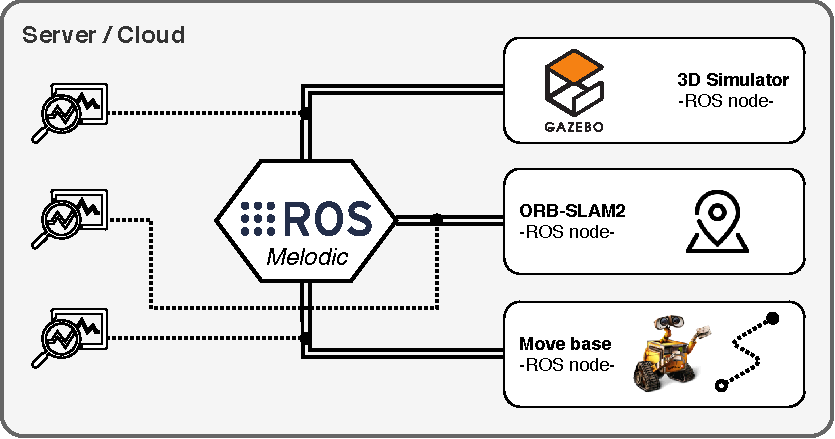
\includegraphics[width=\textwidth]{images/L1-arch-exp}
	\caption{L1 architecture used during the experiments}
	\label{fig:l1archexp}
\end{figure}

Because of the most used robotics platforms used today support the Melodic Morenia \cite{rosmelodic} version of ROS, and because of VOVD was written with the Kinetic version, it has been decided to convert VOVD in the relative Melodic ROS version. This task required a redefinition of some functions related to the ROS \mintinline{cpp}{tf2} package \cite{tfros} due to the deprecation of the \mintinline{cpp}{tf} package functions previously used. 
Another modification done talking about VOVD is related to the 3D map used by Gazebo \cite{Gazebo} simulator. The problem was that it came with a featureless map generated from an ``.urdf'' file, and because of ORB-SLAM2 properly works only if some features are detected during its execution, it has been necessary to add a material to the 3D model of the map.
Talking about ORB-SLAM2, it comes already provided with the necessaries functions to run in a ROS environment, thus no others operations have been required to complete our first architecture level.

Thanks to the modularity of ROS we are able to verify the functional behaviour of the system implementing  a custom ROS node that act as a monitor. It listen on all topics of the system and capture the informations of interest.  
To obtain a more accurate performance measurement, we added some time points within the source code of both VOVD and ORB-SLAM2. Specifically speacking for VOVD we measure the time to perform the local planner computation. To the ORB-SLAM2 side instead we measure the time to elaborate each frame coming frome the simulator camera.
The performance measurement obtained at this architecture level are shown in table \ref{tab:resultL1}.
Note that, due to the modulairy of ROS, we are able to fine tune the system without make any change to the code. For example, we can easily change the frequency of the camera output or the number of the keypoints extracted for each incoming frame.

%TODO queste misuazioni non sono mai state fatte quindi farle al volo e riportare i valori aggiornati nella tabella 

\begin{table}[htbp]
	\begin{tabularx}{\linewidth}{@{}l*{7}{C}c@{}}
		\toprule
		\hline
		Setup              & Odom (ms) & Track Pipe (ms) & Dec. (ms) & Frame Elab. (ms) & Feature Ext.(ms) & Supp. (FPS) \\
		\hline
		\rowcolor{Gray}
		\multicolumn{7}{c}{Performance Measurement: camera 10 Hz}                                                                                                                                           \\
		\hline
		orb(j1)            & -             & 43.41          & 13.08             & 49.21                 & 43.62                  & 20.32           \\ \hline
		vovd(j1)           & 1.70          & -              & -                 & -                     & -                      & -               \\ \hline
		(orb;vovd)(j1)     & 2.58          & 73.49          & 18.69             & 62.70                 & 54.76                  & 13.61           \\ \hline
		(orb(j1);vovd(j2)) & 1.60          & 49.81          & 13.53             & 49.25                 & 43.01                  & 20.08           \\ \hline
		\rowcolor{Gray}
		\multicolumn{7}{c}{Performance Measurement: camera 20 Hz}                                                                                                                                           \\
		\hline
		orb(j1)            & -             & 54.82          & 14.47             & 49.40                 & 44.35                  & 18.24           \\ \hline
		vovd(j1)           & 1.70          & -              & -                 & -                     & -                      & -               \\ \hline
		(orb;vovd)(j1)     & 2.85          & 93.15          & 23.96             & 67.99                 & 60.41                  & 10.74           \\ \hline
		(orb(j1);vovd(j2)) & 1.60          & 56.20          & 14.00             & 49.32                 & 43.95                  & 17.79           \\ \hline
		\bottomrule
\end{tabularx}
\caption{\label{tab:resultL1}Performance measurement at L1 architecture.}
\end{table}

\subsection{Architecture at L2} %TODO Work in progress
Another common architecture in robotics, involves the distribution of ROS nodes on different hardware platforms. In our case we have two NVIDIA Jetson TX2. 
This step requires the split of our system in two parts: the \textit{Host}, on which runs Gazebo simulator, and the \textit{Device/s} that will perform either the robot navigation and SLAM.
Figure \ref{fig:l2arch-exp} show the configuration we setup during the experiment.

\begin{figure}[htbp]
	\centering
	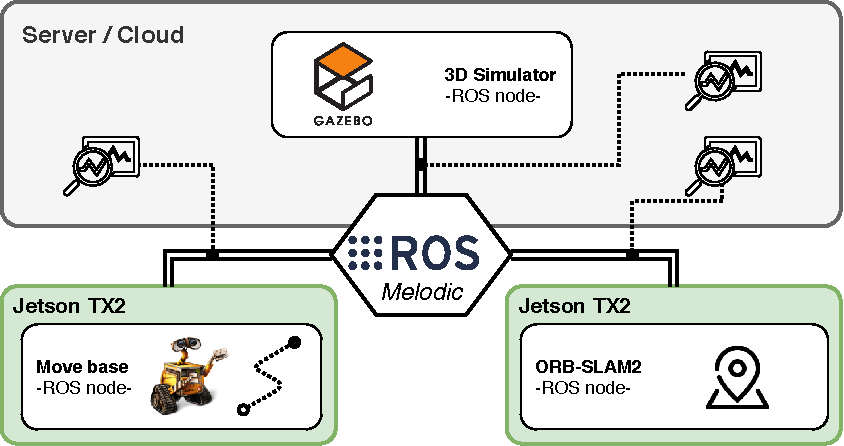
\includegraphics[width=\textwidth]{images/L2-arch-exp}
	\caption{L2 architecture used during the experiments}
	\label{fig:l2arch-exp}
\end{figure}

Due to the several interconnected nodes, each of which having many parameters, it is recommanded create a roslaunch file  using the \textit{machine tag}. As explained in chapter \ref{chap:methodology}, these tags allow control over which nodes run on which machines, for load-balancing and bandwidth management.

At this architecture level the main focus is on the communication between the \textit{Host}, that act as Master, and the other external nodes that represent the slaves. It is important to verify that the system continue working properly and that the Network doesn't become a bottleneck. For example, if we need to transfer a stream of images from one ROS nodes to another that is running on different machine, we should compress each frame before send it over the network. In this way we avoid to saturate the bandwidth of the network. In this case the compression task is performed to the Host side from the aruco camera within Gazebo simulator. The decopression instead is computed on Jetson by the ORB-SLAM2 node whenever it receives a new frame to elaborate.
Once again we measured the performance of the system in the same way we have done in the previous architecture level.
Note that, as we expected, the performance of the ORB-SLAM2 are dropped down due to the computing capability of the Jetson. This is more highligted when we run both VOVD and ORB-SLAM2 on the same device because they are competing for the hardware resources.
The new performance measurements are visible in table \ref{tab:resultL2}.

\begin{table}[htbp]
	\begin{tabularx}{\linewidth}{@{}l*{7}{C}c@{}}
		\toprule
		\hline
		Setup              & Odom (ms) & Track Pipe (ms) & Dec. (ms) & Frame Elab. (ms) & Feature Ext.(ms) & Supp. (FPS) \\
		\hline
		\rowcolor{Gray}
		\multicolumn{7}{c}{Performance Measurement: camera 10 Hz}                                                                                                                                           \\
		\hline
		orb(j1)            & -             & 43.41          & 13.08             & 49.21                 & 43.62                  & 20.32           \\ \hline
		vovd(j1)           & 1.70          & -              & -                 & -                     & -                      & -               \\ \hline
		(orb;vovd)(j1)     & 2.58          & 73.49          & 18.69             & 62.70                 & 54.76                  & 13.61           \\ \hline
		(orb(j1);vovd(j2)) & 1.60          & 49.81          & 13.53             & 49.25                 & 43.01                  & 20.08           \\ \hline
		\rowcolor{Gray}
		\multicolumn{7}{c}{Performance Measurement: camera 20 Hz}                                                                                                                                           \\
		\hline
		orb(j1)            & -             & 54.82          & 14.47             & 49.40                 & 44.35                  & 18.24           \\ \hline
		vovd(j1)           & 1.70          & -              & -                 & -                     & -                      & -               \\ \hline
		(orb;vovd)(j1)     & 2.85          & 93.15          & 23.96             & 67.99                 & 60.41                  & 10.74           \\ \hline
		(orb(j1);vovd(j2)) & 1.60          & 56.20          & 14.00             & 49.32                 & 43.95                  & 17.79           \\ \hline
		\bottomrule
	\end{tabularx}
	\caption{\label{tab:resultL2}Performance measurement at L2 architecture.}
\end{table}



\subsection{Architecture at L3}	%TODO questo non lo abbiamo fatto ma lo mettiamo lo stesso.
Finally we reached the last architecture level of the design flow. It is composed by the \textit{Host}, \textit{Device/s } and the real robot \textit{Robot/s}. In our case the real robot is the KUKA YouBot \cite{YouBot} provided by the robotics laboratory ALTAIR  from university of Verona.



If the previous step have been properly done, this one should be completely 
transparent with respect to the entire system. 
As we can see in Fig. \ref{fig:l3archexp}, the simulator has been removed from the \textit{Host} and it is replaced by the real robot, on which one or more embedded devices are attached.
To achieve this goal ... 
%TODO chiedere a piccinelli qual'è la modifica da fare per eseguire i comandi sul robot anziché sul simulatore


\begin{figure}
	\centering
	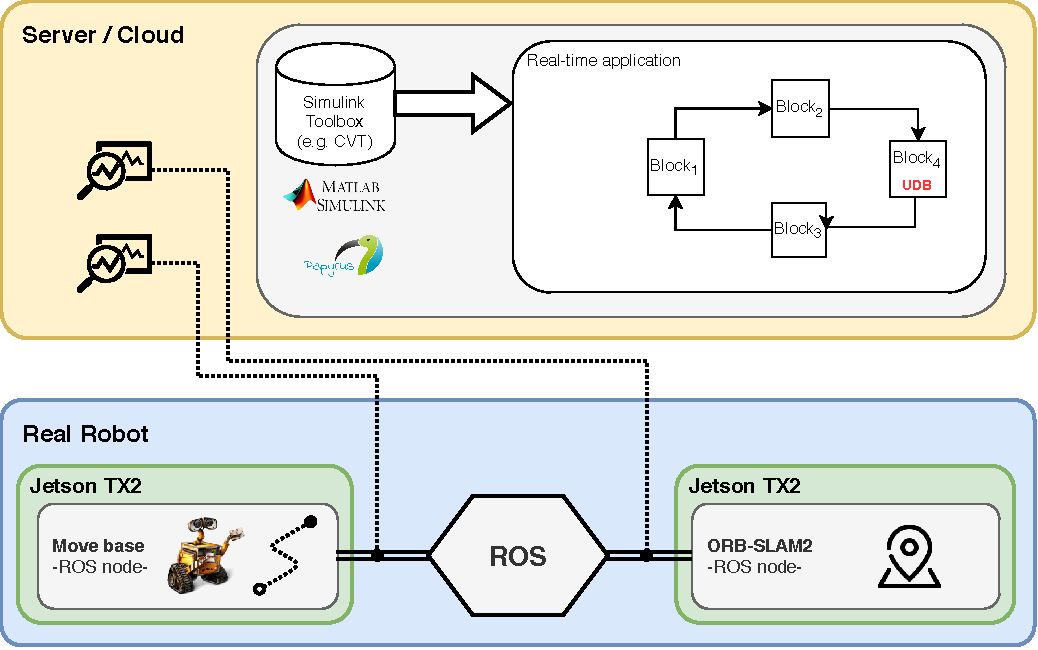
\includegraphics[width=\textwidth]{images/L3-arch}
	\caption{L3 architecture}
	\label{fig:l3archexp}
\end{figure}


\section{Deployment from the cloud to the edge} % How to prepare an application for edge computing in Kubeedge?
As mentioned in \ref{kubeedgebackground}, Kubeedge is built upon Kubernetes and provides fundamental infrastructure support for network, app. deployment and metadata synchronization between cloud and edge. As we know, Kubernetes uses containers to run isolated, packaged applications across its cluster nodes. To run on Kubernetes, your applications must be encapsulated in one or more container images and executed using a container runtime like Docker. While containerizing your components is a requirement for Kubernetes, it also allow easy scaling and management. For instance, containers provide isolation between the application environment and the external host system, support a networked, service-oriented approach to inter-application communication, and typically take configuration through environmental variables and expose logs written to standard error and standard out. Containers themselves encourage process-based concurrency and help maintain dev/prod parity by being independently scalable and bundling the process’s runtime environment. These characteristics make it possible to package your applications so that they run smoothly on Kubernetes. In this section it will described the process used in our project to prepare both VOVD and ORB-SLAM2 applications for the edge computing through the support of Kubeedge.


\subsection{VOVD at the edge}
%TODO Dockerfile di VOVD 
%TODO Problemi in fase di building del container --> ROS network comunication


\subsection{ORB-SLAM2 at the edge}
%TODO Dockerfile di ORB_SLAM2 
%TODO Problemi in fase di building del container --> ROS + GPU (TRT)

\section{The whole system on Kubeedge}
%TODO Once we have containerized our applications we are ready to deploy them from the cloud to the edge with kubeedge: L1, L2, L3 ?!.



\section{Discussion}

















































\subsection{Hybrid local/global planner}



\section{Results}
%\begin{table}[ht!]
%	\resizebox{\linewidth}{!}{%
%		\begin{tabular}{|l|c|c|c|c|c|c|c|c|c|} 
%			\hline
%			\hspace{3mm} Setup & Odom VOVD (ms) & Track Pipe (ms) & Decompression (ms) & Frame Elaboration (ms) & Feature Extraction (ms) & Supported (FPS)  \\ 
%			\hline
%			\rowcolor{Gray}
%			\multicolumn{7}{|c|}{Performance Measurement: camera 10 Hz}  \\
%			\hline
%			orb(j1)     					 &	-  		  & 43.41 & 13.08  & 49.21 & 43.62 & 20.32   \\ \hline
%			vovd(j1)       	 			  & 1.70  & -     	 	 & -    		 & -     		& -    		   & -     		  \\ \hline
%			(orb;vovd)(j1)      	& 2.58 	& 73.49 & 18.69  & 62.70 & 54.76  & 13.61 	 \\ \hline
%			(orb(j1);vovd(j2))  & 1.60 	& 49.81 & 13.53  & 49.25 & 43.01  & 20.08	 \\ \hline
%			\rowcolor{Gray}
%			\multicolumn{10}{|c|}{Performance Measurement: camera 20 Hz}  \\
%			\hline
%			orb(j1)     					 &   -  	 & 54.82 & 14.47 & 49.40 & 44.35 &18.24 	 \\ \hline
%			vovd(j1)       	 			  & 1.70 & -     		& -     	   & -     		 & -     		& -     			 \\ \hline
%			(orb;vovd)(j1)      	& 2.85 & 93.15 & 23.96 & 67.99 & 60.41 & 10.74 		\\ \hline
%			(orb(j1);vovd(j2))  & 1.60 & 56.20 & 14.00 & 49.32 & 43.95 & 17.79 		\\ \hline
%			\rowcolor{Gray}
%			\multicolumn{7}{|c|}{Kubeedge - Performance Measurement: camera 10 Hz}  \\
%			\hline
%			orb(j1)     					& -    		 & 47.28 & 12.78  & 40.52 & 36.02 & 21.15 	 \\ \hline
%			vovd(j1)       	 			  & 1.30 & -     		& -     	   & -     		  & -     		 & -     		   \\ \hline
%			(orb;vovd)(j1)      	& 1.40 & 82.47 & 15.10  & 53.54 & 48.09 & 12.12		\\ \hline
%			(orb(j1);vovd(j2))  & 1.38 & 50.83 & 13.98  & 43.80 & 38.04 & 19.67		\\ \hline
%			\rowcolor{Gray}
%			\multicolumn{7}{|c|}{Kubeedge - Performance Measurement: camera 20 Hz}  \\
%			\hline
%			orb(j1)     					 & -    	 & 50.20 & 16.20 & 42.16 & 34.82 & 19.92  \\ \hline
%			vovd(j1)       	 			  & 1.21 & -			& -     	   & -     		 & -     		& -     		\\ \hline
%			(orb;vovd)(j1)      	& 1.43 & 70.54 & 15.02  & 55.60 & 50.24 & 14.18  \\ \hline
%			(orb(j1);vovd(j2))  & 1.26 & 58.14 & 13.52  & 42.34 & 37.17 & 17.20  \\ \hline
%	\end{tabular}}
%	\caption{Performance Measurement\label{tab:Performance-Measurement}}
%\end{table}





\begin{table}[hbt]
	\begin{tabularx}{\linewidth}{@{}l*{7}{C}c@{}}
		\toprule
		\hline
		Setup              & Odom (ms) & Track Pipe (ms) & Dec. (ms) & Frame Elab. (ms) & Feature Ext.(ms) & Supp. (FPS) \\
		\hline
		\rowcolor{Gray}
		\multicolumn{7}{|c|}{Performance Measurement: camera 10 Hz}                                                                                                                                           \\
		\hline
		orb(j1)            & -             & 43.41          & 13.08             & 49.21                 & 43.62                  & 20.32           \\ \hline
		vovd(j1)           & 1.70          & -              & -                 & -                     & -                      & -               \\ \hline
		(orb;vovd)(j1)     & 2.58          & 73.49          & 18.69             & 62.70                 & 54.76                  & 13.61           \\ \hline
		(orb(j1);vovd(j2)) & 1.60          & 49.81          & 13.53             & 49.25                 & 43.01                  & 20.08           \\ \hline
		\rowcolor{Gray}
		\multicolumn{7}{|c|}{Performance Measurement: camera 20 Hz}                                                                                                                                           \\
		\hline
		orb(j1)            & -             & 54.82          & 14.47             & 49.40                 & 44.35                  & 18.24           \\ \hline
		vovd(j1)           & 1.70          & -              & -                 & -                     & -                      & -               \\ \hline
		(orb;vovd)(j1)     & 2.85          & 93.15          & 23.96             & 67.99                 & 60.41                  & 10.74           \\ \hline
		(orb(j1);vovd(j2)) & 1.60          & 56.20          & 14.00             & 49.32                 & 43.95                  & 17.79           \\ \hline
		\rowcolor{Gray}
		\multicolumn{7}{|c|}{Kubeedge - Performance Measurement: camera 10 Hz}                                                                                                                                \\
		\hline
		orb(j1)            & -             & 47.28          & 12.78             & 40.52                 & 36.02                  & 21.15           \\ \hline
		vovd(j1)           & 1.30          & -              & -                 & -                     & -                      & -               \\ \hline
		(orb;vovd)(j1)     & 1.40          & 82.47          & 15.10             & 53.54                 & 48.09                  & 12.12           \\ \hline
		(orb(j1);vovd(j2)) & 1.38          & 50.83          & 13.98             & 43.80                 & 38.04                  & 19.67           \\ \hline
		\rowcolor{Gray}
		\multicolumn{7}{|c|}{Kubeedge - Performance Measurement: camera 20 Hz}                                                                                                                                \\
		\hline
		orb(j1)            & -             & 50.20          & 16.20             & 42.16                 & 34.82                  & 19.92           \\ \hline
		vovd(j1)           & 1.21          & -              & -                 & -                     & -                      & -               \\ \hline
		(orb;vovd)(j1)     & 1.43          & 70.54          & 15.02             & 55.60                 & 50.24                  & 14.18           \\ \hline
		(orb(j1);vovd(j2)) & 1.26          & 58.14          & 13.52             & 42.34                 & 37.17                  & 17.20           \\ \hline
		\bottomrule
	\end{tabularx}
	\caption{\label{tab:Performance-Measurement2}Performance Measurement.}
\end{table}







%%%%%%%%%%%%%%%%%%%%%%5
\clearpage
\thispagestyle{empty}